\documentclass[a4paper]{article}
\usepackage[english]{babel}
\usepackage[utf8]{inputenc}

%
% Graphics
%
\usepackage{graphicx}
\usepackage{xcolor}

\definecolor{alpha}{HTML}{3FA9F5}

%
% Bibliography
%
\usepackage[backend=bibtex,maxnames=5,sorting=none,url=false]{biblatex}
\usepackage{csquotes}

%
% Listings
%
\usepackage{listings}

\definecolor{background}{HTML}{FAFAFA}
\definecolor{sign}{HTML}{3FA9F5}

\lstdefinelanguage{fortune}{
  basicstyle=\ttfamily,
  basewidth={0.5em,0.5em},
  backgroundcolor=\color{background},
  literate=
   *{\%}{{{\color{alpha}{\%}}}}{1}
}

\lstdefinelanguage{shell}{
  basicstyle=\ttfamily,
  basewidth={0.5em,0.5em},
  backgroundcolor=\color{background},
  literate=
    [*]{\\\$}{{{\color{alpha}{\$}}}}{1}
       {Command>}{{{\color{alpha}{Command>}}}}{8}
       {ivan(0)>}{{{\color{alpha}{ivan(0)>}}}}{8}
       {ivan(1)>}{{{\color{alpha}{ivan(1)>}}}}{8}
       {ivan(0):RELEASED>}{{{\color{alpha}{ivan(0):RELEASED>}}}}{17}
       {ivan(0):LOCKED>}{{{\color{alpha}{ivan(0):LOCKED>}}}}{15}
       {ivan(1):LOCKED>}{{{\color{alpha}{ivan(1):LOCKED>}}}}{15}
       {ivan(2):LOCKED>}{{{\color{alpha}{ivan(2):LOCKED>}}}}{15}
}

\lstdefinelanguage{json}{
  basicstyle=\ttfamily,
  basewidth={0.5em,0.5em},
  backgroundcolor=\color{background},
  literate=
   *{:}{{{\color{alpha}{:}}}}{1}
    {,}{{{\color{alpha}{,}}}}{1}
    {\{}{{{\color{alpha}{\{}}}}{1}
    {\}}{{{\color{alpha}{\}}}}}{1}
    {[}{{{\color{alpha}{[}}}}{1}
    {]}{{{\color{alpha}{]}}}}{1}
}

\lstnewenvironment{fortune}%
{\lstset{language=fortune}}%
{}

\lstnewenvironment{json}%
{\lstset{language=json}}%
{}

\lstnewenvironment{shell}%
{\lstset{language=shell}}%
{}

%
% Links
%
\usepackage{hyperref}
\hypersetup{%
  colorlinks=true,
  citecolor={alpha},
  linkcolor={alpha},
  urlcolor ={alpha}
}

%
% Text
%
\newcommand{\ie}{i.e.}
\newcommand{\eg}{e.g.}
\newcommand{\etc}{etc.}

\newcommand{\fix}{should be modified}
\newcommand{\leave}{no changes are needed}
\newcommand{\overwrite}{should contain your previous changes}

\newcommand{\python}{\texttt{Python}}
\newcommand{\classname}[1]{\texttt{#1}}
\newcommand{\filename}[1]{\texttt{#1}}
\newcommand{\code}[1]{\texttt{#1}}

%
% References
%
\newcommand{\sref}[1]{Section~\ref{sec:#1}}
\newcommand{\tref}[1]{Table~\ref{tab:#1}}
\newcommand{\fref}[1]{Figure~\ref{fig:#1}}

\newcommand{\slabel}[1]{\label{sec:#1}}
\newcommand{\tlabel}[1]{\label{tab:#1}}
\newcommand{\flabel}[1]{\label{fig:#1}}

\newcommand{\slab}[1]{\label{sec:#1}}
\newcommand{\tlab}[1]{\label{tab:#1}}
\newcommand{\flab}[1]{\label{fig:#1}}

\newcommand{\aref}[1]{Lab~#1 \cite{description#1}}


\bibliography{include/references.bib}

\title{%
  Distributed Systems: Lab 2\\%
  Middleware: Object Request Brokers%
}
\author{Petru Eles and Adrian Horga\\
\vspace{0.5em}
\href{mailto:petru.eles@liu.se}{petru.eles@liu.se} and
\href{mailto:adrian.horga@liu.se}{adrian.horga@liu.se}
}
% \date{December 27, 2016}

\begin{document}
\maketitle

\section{Introduction}
\begin{figure}
  \centering
  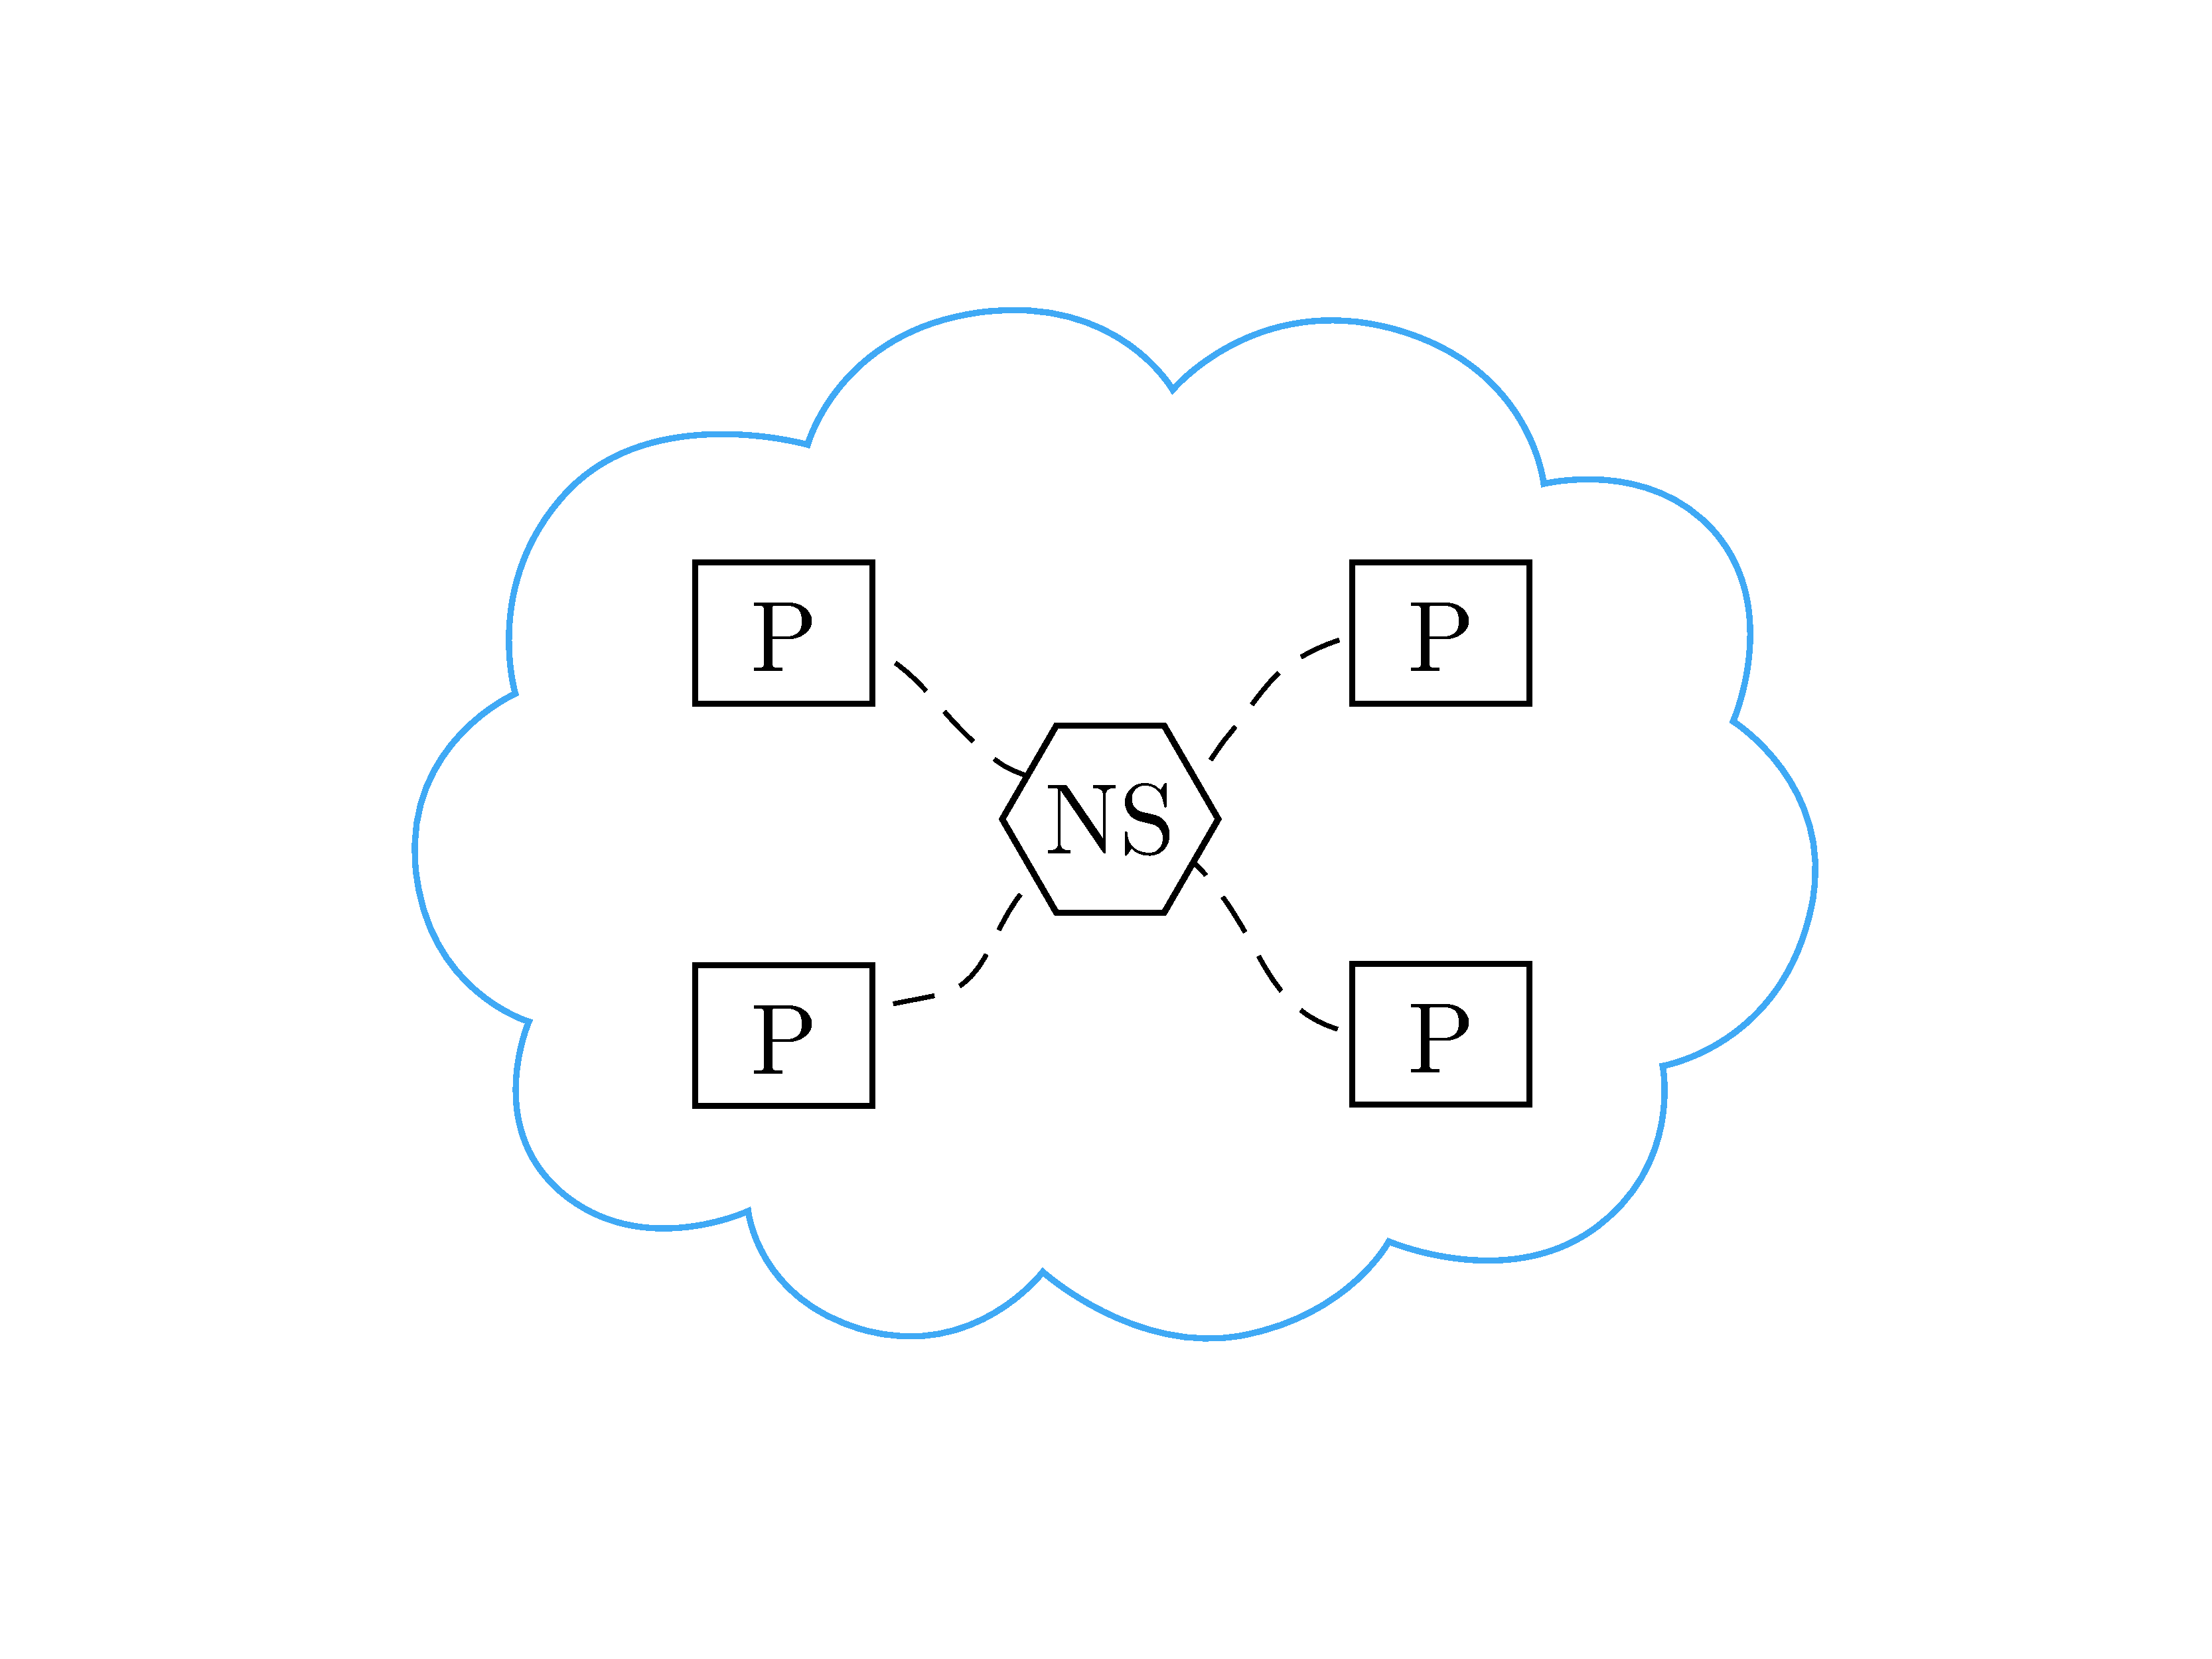
\includegraphics[width=0.8\textwidth, clip=true, trim=0 180px 0 180px]{include/assets/name-service.pdf}
  \caption{A number of peers (P), equipped with object request brokers, discovering each other through a name service (NS).}
  \flabel{name-service}
\end{figure}

In the previous lab, you implemented a distributed system with a single server
and an arbitrary number of clients. The clients were required to explicitly
specify the hostname and port of the server in order to interact with the
database. It was not convenient as this information could easily change. The
situation becomes significantly more complicated when there are many servers
joining and leaving the network in an arbitrary way. Such a freedom is at heart
of a distributed system, and it is exactly what we aim to achieve by the end of
the programming project. In this lab, you will implement the code that will
allow the participants of your distributed system to smoothly discover each
other. At this point, we shift our focus from the client-server to peer-to-peer
model \cite{lecture3} and refer to participants as peers.

The problem outlined above is solved by introducing into our distributed system
a so-called middleware \cite{lecture4}; carefully read the corresponding
sections in \cite{lecture4} to get a better understanding of the lab. Loosely
speaking, a middleware of a distributed system is an auxiliary layer that hides
all the complexity of the communication process between peers. Such a layer is
typically divided into two parts: object services (\eg, name services) and
object request brokers.

A name service is a global registrar of all the objects/peers that participate
in the network. Upon request, a name service can, for instance, provide
information about the current location of a particular peer; this scenario is
depicted in \fref{name-service}. For our purposes, it is sufficient to assume
that the name service is unique, it is reliable, and its address is fixed and
known to everyone.

An object request broker \cite{lecture4, orb} is a piece of code on a peer's
side that interacts with a name service and creates an illusion for the peer
that other peers---which might be running on different machines and/or in
different processes on the same machine---are running in separate threads of
this peer. In other words, it creates an impression that everything is local to
the peer, and there is no need of any network communications, which is very
convenient.

A name service is already present in the LiU network for you to use. The source
code of the name service will not be given; however, the interface of this
machine will be described (see \sref{interface}) such that you can employ it for
your purposes by sending adequate messages. Consequently, your first task is to
learn how to interact with this auxiliary component. To this end, in this lab,
you will put aside your previous code and implement a simple application with
the only purpose of registering in the name service and listing the addresses of
the peers that are currently present in the network. This knowledge will help
you to seamlessly incorporate the name service into your distributed database of
fortunes in the future labs.

\section{Name Service Interface} \slab{interface}
The foremost aspect to note is that the name service is following the
communication protocol introduced in \aref{1}. Thus, the remote method
invocation mechanism of the name service is also based on JSON-encoded messages.
The interface has of the following methods accessible to peers:
\begin{itemize}

  \item \code{register} --- registers a peer in the name service and returns two
  identifiers assigned to the peer for the future reference (see the next
  method);

  \item \code{unregister} --- unregisters a peer in the name service using the
  two identifiers obtained by calling \code{register};

  \item \code{require\_all} --- retrieves the list of the registered peers of a
  given object type (object types are explained below).

\end{itemize}
These methods are already being properly called in the provided source code
(however, the actually transfer of the associated messages is yet to be fixed by
you). Therefore, we leave it to you to find those places in the code and further
investigate the input and output arguments of the three methods.

Since there is only one name service for all the students, several students can
interfere with each other. In order to prevent this, the name service has been
designed in such a way that each student can work within a separate name space.
Each name space is characterized by a unique identifier, which we shall refer to
as an object type (each peer is an object, and a name space contains all objects
of a given type). This unique identifier is to be specified by you in a special
file (namely, in \filename{objectType.py} as you will see in \sref{task}). As
the name suggests, you should choose something unique, \eg, your student ID. You
can also experiment with other students (but do not forget to tell them
beforehand) by joining several networks together, which can be achieved by
sharing the same object type; otherwise, keep your object type secret.

\section{Your Task} \slab{task}
\subsection{Preparation}
Continue working with the same code base that you have been working with so far,
including all the changes that you have made. The files relevant to this lab are
listed below. You should read and understand them.
\begin{itemize}

  \item \filename{lab2/peer.py} --- the \classname{Peer} application (\leave);

  \item \filename{lab2/test.sh} --- a shell script that you can use for testing;

  \item \filename{modules/Common/nameServiceLocation.py} --- the file that
  contains the address of the name service (\leave);

  \item \filename{modules/Common/objectType.py} --- the file that defines the
  object type of your peers registered in the name service as explained in
  \sref{interface} (\fix);

  \item \filename{modules/Common/orb.py} --- the code of your object request
  broker (\fix);

  \item \filename{modules/Common/wrap.sh} --- the same as for \aref{1}.

\end{itemize}
Go through the code and grasp the main idea behind each part. You can also try
to run the main executable file of the lab, that is, \filename{peer.py}, and you
will observe that the application cannot even start without your help.

\subsection{Understanding the Setup}
Let us focus on the module \filename{orb.py} that contains an incomplete
implementation of an object request broker \cite{lecture4}. The module includes:
\begin{itemize}

  \item \classname{Stub} --- the class that represents the image of a remote
  object on the local machine (therefore, it is also called a proxy); the main
  purpose of the class is remote method invocation \cite{lecture3}.

  \item \classname{Skeleton} --- the class that is used to listen to incoming
  connections and forward them to an instance of the \classname{Peer} class.

  \item \classname{Peer} --- the class that implements basic bidirectional
  communications using \classname{Stub} and \classname{Skeleton}; any object
  willing to interact with remote objects should extend this class, which is
  what is done in \filename{peer.py}.

\end{itemize}

Now we shall describe how object request brokers work considering a special case
wherein a peer interacts with the name service; the same logic applies to
communications between two arbitrary peers. Recall that the name service is
running on a separate machine in the network. A local representation of the name
service is given by the \code{name\_service} instance variable of the
\classname{Peer} class. This variable is initialized as an instance of the
\classname{Stub} class, which can be viewed as an image of the name service on
the local machine. All this image does (or is supposed to do after you complete
the implementation) is the forwarding across the network of incoming method
invocations to the name service (the real one).

\classname{Stub} undertakes the aforementioned forwarding is a very general way,
which can be summarized as follows. In \python, whenever you call a missing
method of an object, an implicit call to the object's \code{\_\_getattr\_\_}
method \cite{python-getattr} is done. \code{\_\_getattr\_\_} exists in all
\python\ objects, and it raises an exception by default. In \classname{Stub},
however, this handy method is overwritten in order to generate and return the
requested method on the fly. This generated method simply forwards the call to
the real object via \python's sockets, which you got familiar with in \aref{1}.
The whole idea of \classname{Stub} is to act as an image of any remote object
and, thus, to imitate any remote interface. Thus, the three methods listed in
\sref{interface} exist in the name service located somewhere in the network, and
\classname{Stub} generates these methods for the client when they are needed.

The \classname{Skeleton} class also plays an important role in our distributed
system. In particular, it allows the name service for a proper maintenance of
the list of active peers. Whenever a peer leaves the network and unregisters
itself, the name service pings the rest of the peers to see whether they are
still alive. It is done by calling the \code{check} method of the
\classname{Peer} class, and, if a peer does not reply properly, the name
services removes it from the list of active peers. Consequently, without a
correct implementation of \classname{Skeleton}, which is supposed to forward
incoming requests to \classname{Peer}, all your peers might be removed from the
active list of the name service, and a new peer will not see them.

\subsection{Implementation}
Now you are ready to complete the implementation of the object request broker in
\filename{orb.py}, namely, the classes \classname{Stub}, \classname{Skeleton},
and \classname{Peer}. As before, you are supposed to implement the functions
marked with ``Your code here.''

The requirements are similar to those given in \aref{1}:
\begin{itemize}

  \item The communication protocol that you should maintain is the one described
  in \aref{1}.

  \item Your peers should adequately handle exceptions (due to potential network
  problems, violations of the protocol, invocations of non-existing functions,
  invocations of proper functions but with wrong arguments, \etc).

  \item Whenever a peer receives an error in response to a method call, it
  should instantiate and raise this error as if it has occurred locally.

\end{itemize}
As you remember, each remote method invocation should be encoded in JSON and
sent to the remote side, which is always the name service in this lab. In this
regard, pay your attention to the \code{\_rmi} function in \classname{Stub}. The
name service returns the result of the call as a JSON-encoded object containing
the output of the method, if it was successful, or an error, if the execution
failed.

Have a look at the arguments passed to \code{register} (see \sref{interface}). A
common problem is that \code{socket.gethostname()} in \filename{peer.py} is
unable to detect the IP address of your machine, in which case the function
yields \code{127.0.0.1} or alike and the name service receives rather
meaningless information about the peer. A workaround is to hardcode your IP
address in \filename{peer.py}.

After a successful completion of the lab, each new peer started in a new
terminal window should output its own address and the addresses of all other
peers that have already been started and have not been terminated. However,
those other peers will not (and, in this lab, are not supposed to) see the new
one. Remember that you are provided with a test script
(\filename{lab2/test.sh}), which can set up everything for you.

\section{Conclusion}
Having completed the lab, you have made an important step towards your
distributed database of fortunes: now you have an object request broker that can
properly interact with the name service (and, actually, with other peers).
However, the simple listing of available peers achieved so far is not something
extremely useful by itself. Moreover, as it was discussed at the end of the
previous section, each peer is aware only of those participants that joined the
system before it. In addition, if a peer leaves the network, the other machines
will not notice this change and, thus, can be misled. Therefore, in the next
lab, you will (a) extend the application constructed here to call some useful
functions of other peers (not only of the name service) and (b) implement an
auxiliary class that will help to properly maintain the list of active peers.

\printbibliography

\end{document}
